\section{$\Delta$Q display}
    An probe's displayed graph must contain the following functions:
    \begin{itemize}
        \item The mean and confidence bounds of a window of previous $\Delta$Qs.
        \item The observed $\Delta$Q($t_l, t_u, dMax$).
        \item If applicable, the calculated $\Delta$Q from the components showing the causal links of a probe.
        \item Its QTA (if defined).
    \end{itemize}
    This allows for the user to observe if a $\Delta$Q has deviated from normal execution, analyse its stationarity, nonlinearity and observe its execution.
    \iffalse 
    \begin{figure}[!ht]    
    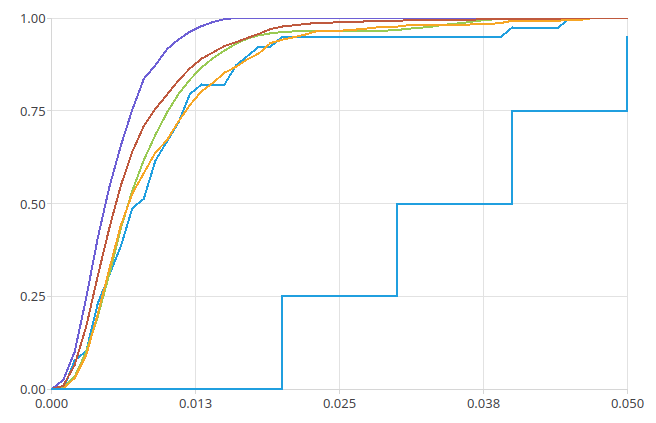
\includegraphics[scale =0.8, width=\textwidth]{img/dqdispl.png}
    \end{figure}
    \fi
